%----------------------------------------
% Preamble to set up the document
%----------------------------------------
\documentclass{article}

% set up packages (you shouldn't need to touch this)
\usepackage{graphicx}  % required to insert images
\usepackage{hyperref}  % for hyperlinks
\usepackage[svgnames]{xcolor}  % to change hyperlink colors
\colorlet{linkcolour}{DarkBlue}
\hypersetup{colorlinks=true, linkcolor=linkcolour, citecolor=linkcolour, urlcolor=linkcolour,}

% Margins
\topmargin=-0.45in
\evensidemargin=0in
\oddsidemargin=0in
\textwidth=6.5in
\textheight=9.0in
\headsep=0.25in

% use a sans serif font
\renewcommand{\familydefault}{\sfdefault}

%----------------------------------------
% Step 1: Edit the lecture title
%----------------------------------------
\title{
Lecture 10: Networks (Counting on steroids) \\  % Lecture title
Modeling Social Data, Spring 2017 \\   % Course title
Columbia University                    % School
}

%----------------------------------------
% Step 2: Edit your name and the date
%----------------------------------------
\author{Chris Lam}                     % Scribe's name
\date{April 7, 2017}                % Lecture date

\begin{document}

\maketitle


%----------------------------------------
% Step 3:
% Rename uni.tex to match your uni,
% edit the filename accordingly below,
% and put your notes in this file
%----------------------------------------

%----------------------------------------
% Write your notes here
%----------------------------------------

\section{On Networks}
\subsection{History}
\begin{itemize}
  \item '30s: Breaking news: Networks are a thing!
  \item '60s: Random graph theory: Erdos + Rengi ('59)
  \begin{itemize}
	\item thought of graphs as math, as objects to be studied
	\item high probability:  more clustered in one component
	\item low probability: more scattered across multiple components
  \end{itemize}
  \item '70s: Granovetter ('73): Clustering and weak ties
  \begin{itemize}
	\item The friends of my friends are often friends.
    \begin{figure}[ht]
    	\begin{center}
      	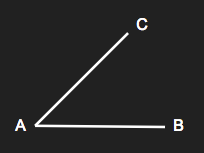
\includegraphics[width=0.2\textwidth]{figures/Figure_1_Granovetter.png}
      	\caption{
        	Granovetter: this is forbidden; it's impossible for A-C and A-B to be the case without B-C being a thing as well!}
    	\label{fig:figure1}
  		\end{center}
	\end{figure}
	\item Ties can be strong (triadic closure) or weak (bridges).
    \item I may not know too well the people who bridge me to other 		communities.
  \end{itemize}
  \item '70s - relatively recently: Cross-platform data outside of surveys for social networks isn't lying around, making it hard to study.
  \item '70s: de Solla Price ('65,'76): Cumulative advantage in citation networks -- in many other words:
	\begin{itemize}
		\item Uneven distribution of attention
		\item Popularity begets itself
		\item There are a few celebrities and a bunch of nobodies.
  	\end{itemize} 
  \item '90s: Watts + Strogatz ('98): Small-world networks
  	\begin{itemize}
		\item Randomly rewired edges of a regular network
		\item Bridged the gap between IRL and the completely random graph
		\item Featured short path lengths (ie. just a few hops from A to B), triadic closure, and bridging
  	\end{itemize} 
    \item '00s: Newman, Barabusi, Watts ('06): Empirical structure from actual data, ie. hairballs
    	\begin{itemize}
		\item Adamic + Glance ('05): Homophily        
		\item Warning: location of nodes (blogs) may be contrived.
		\item Favors the lowest-energy configuration: force-directed, springlike edges that collapse close-together nodes more densely together in parameter space.
  	\end{itemize} 
\end{itemize}


\subsection{Types of networks}
Networks are abstractions of different types of data. We can be handed social (think: Facebook), informational (think: the web, political blogs, citations), activity (think: email), biological, and even geographical (think: roads) networks. It's important not to lose sight of what's being abstracted to a network. 

Representations, ie. levels of abstraction
\begin{itemize}
	\item Undirected
    	\begin{figure}[ht]
    		\begin{center}
      	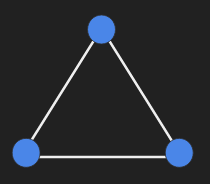
\includegraphics[width=0.2\textwidth]{figures/Undirected_friends.png}
      	\caption{
        	Bidirectional friendship (one would hope)}
    	\label{fig:figure3}
  			\end{center}
		\end{figure}
    \item Directed
    	\begin{figure}[ht]
    		\begin{center}
      	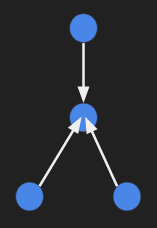
\includegraphics[width=0.15\textwidth]{figures/Directed_pg_followers.png}
      	\caption{
        	Directed network, eg. followers of a FB page}
    	\label{fig:figure4}
  			\end{center}
		\end{figure}
   \item Weighted (the old ARPAnet, the OG Internet, whose edge costs varied)
   \item Metadata: attributes of the nodes and edges themselves
   \item Ego networks: by changing the threshold for what constitutes a 'meaningful' interaction or relationship, we change what the network looks like. 'All my FB friends', for example, will be much denser than 'my carefully maintained relationships'.  
\end{itemize} 

\subsection{Data Structures of Networks}
\begin{itemize}
	\item Edge list: storage :) compute :(
    	\begin{itemize}
		\item Compute time $\propto$ number of edges     
		\item To check if edge is present, requires a big scan, linear through number of edges
  		\end{itemize} 
    \item Adjacency matrix: checking edges :) linear algebra :) 
    	\begin{itemize}
        \item Storage in a sparse matrix is more efficient
		\item The not as big scan: run down the row or column; but this gets less easy for directed graphs because the matrix for these aren't symmetric
        \item Compute time $\propto$ number of nodes  
  		\end{itemize} 
    \item Adjacency list: graph traversal :) 
    	\begin{itemize}
        \item Compute time $\propto$ average number of neighbors for all nodes
  		\end{itemize}     
\end{itemize}

Descriptive Stats of Networks: 
\begin{center}
    \begin{tabular}{| l | l | l |}
    \hline
    Stat & Definition & Associated algorithm \\ \hline
    Degree & \# connections a node has & Degree distributions (counting) \\ \hline
    Path length & Shortest path between 2 nodes & BFS \\ \hline
    Clustering & How many friends of friends are also friends? & Triangle counting \\ \hline
    Components & \# disconnected parts & Connected components \\
    \hline
    \end{tabular}
\end{center}


\subsection{Coding up Networks}






\end{document}

%%% Local Variables:
%%% mode: latex
%%% TeX-master: t
%%% End:
